%% DONE
\id{МРНТИ 06.77.65}{https://doi.org/10.58805/kazutb.v.1.26-566}

\begin{articleheader}
\sectionwithauthors{S.K. Zhumashbekova, B.M. Bayadilova, A.S. Koichubayev}{YOUTH MIGRATION AND THE QUALITY OF HUMAN CAPITAL}

{\bfseries
\textsuperscript{1}S.K. Zhumashbekova\alink{https://orcid.org/0000-0003-1119-6478},
\textsuperscript{2}B.M. Bayadilova\alink{https://orcid.org/0000-0002-4972-3408},
\textsuperscript{3}A.S. Koichubayev\textsuperscript{\envelope } \alink{https://orcid.org/0000-0002-2814-9419}}
\end{articleheader}

\begin{affiliation}
\emph{\textsuperscript{1}Shakarim University, Semey, Kazakhstan,}

\emph{\textsuperscript{2}K.Kulazhanov Kazakh University of Technology and Business, Astana, Kazakhstan,}

\emph{\textsuperscript{3}Alikhan Bokeikhan University, Semey, Kazakhstan,}

\raggedright \textsuperscript{\envelope }{\em Corresponding author: koichubayev.a@abu.edu.kz}
\end{affiliation}

This article examines the impact of youth migration on the quantitative
and qualitative parameters of human capital. Using the example of
Kazakhstan, the features of external youth migration, which have a
positive and negative impact on the human capital of the receiving and
giving country, were studied. In this study, methods of quantitative and
qualitative analysis and the graphical method of economic research are
used. The authors noted that the most important determinants of leaving
the country are education and employment. It was determined that the
main share of young migrants in the total structure of migration flows
from Kazakhstan left for the Russian Federation, and the main reasons
for this situation were established. The pushing and attracting factors
stimulating the migration of young people have been identified by
interviewing respondents abroad using social networks and messengers.
The importance of the economic consequences of the migration of human
capital is also considered, it is noted that in many ways the
consequences of the departure of highly qualified labor depend on the
level of development of the state and the state of the national economy.
The Concept of migration policy of the Republic of Kazakhstan until 2027
is considered, where one of its key areas is educational migration, and
initiatives will be implemented within this area, including attracting
highly qualified specialists to the country.

{\bfseries Keywords:} migration processes, youth migration, human capital,
migration gain, educational migration, labor migration.

\begin{articleheader}
{\bfseries ЖАСТАР КӨШІ-ҚОНЫ ЖӘНЕ АДАМИ КАПИТАЛДЫҢ САПАСЫ}

{\bfseries
\textsuperscript{1}С.К. Жумашбекова,
\textsuperscript{2}Б.М. Баядилова,
\textsuperscript{3}А.С. Койчубаев\textsuperscript{\envelope }}
\end{articleheader}

\begin{affiliation}
\emph{\textsuperscript{1}Шәкәрім атындағы университеті, Семей, Қазақстан,}

\emph{\textsuperscript{2}Қ.Құлажанов атындағы Қазақ технология және бизнес университеті, Астана, Қазақстан,}

\emph{\textsuperscript{3}Alikhan Bokeikhan University, Семей, Қазақстан,}

\emph{e-mail: koichubayev.a@abu.edu.kz}
\end{affiliation}

Бұл мақалада жастар көші-қонының адами капиталдың сандық және сапалық
параметрлеріне әсері қарастырылған. Қазақстан мысалында қабылдаушы және
шығарушы елдің адами капиталына оң және теріс әсер ететін сыртқы жастар
көші-қонының ерекшеліктері зерттелді. Бұл зерттеуде сандық және сапалық
талдау әдістері, экономикалық зерттеулердің графикалық әдісі қолданылды.

Авторлар елден кетудің маңызды детерминанттары білім алу және жұмысқа
орналасу болып табылатынын атап өтті. Қазақстаннан Ресей Федерациясына
көші-қон ағындарының жалпы құрылымындағы жас мигранттардың негізгі үлесі
кеткені анықталды, бұл жағдайдың негізгі себептері анықталды. Шетелде
жүрген респонденттерден әлеуметтік желілер және мессенджерлер арқылы
сұхбат алынып, жастардың көші-қонын ынталандыратын және тартатын
факторлар анықталды. Сондай-ақ, адами капитал көші-қонының экономикалық
салдарының маңыздылығы қарастырылды, көп жағдайда жоғары білікті жұмыс
күшінің кетуінің салдары мемлекеттің даму деңгейіне және ұлттық
экономиканың жағдайына байланысты екендігі атап өтілді. Қазақстан
Республикасының 2027 жылға дейінгі көші-қон саясатының тұжырымдамасы
қаралды, онда оның негізгі бағыттарының бірі білім беру көші-қоны болып
табылады және осы бағыт шеңберінде бастамалар, оның ішінде елге жоғары
білікті мамандарды тарту іске асырылатыны айтылды.

{\bfseries Түйін сөздер:} көші-қон процестері, жастар көші-қоны, адами
капитал, көші-қон өсімі, білім беру көші-қоны, еңбек көші-қоны.

\begin{articleheader}
{\bfseries МОЛОДЕЖНАЯ МИГРАЦИЯ И КАЧЕСТВО ЧЕЛОВЕЧЕСКОГО КАПИТАЛА}

{\bfseries
\textsuperscript{1}С.К. Жумашбекова,
\textsuperscript{2}Б.М. Баядилова,
\textsuperscript{3}А.С. Койчубаев\textsuperscript{\envelope }}
\end{articleheader}

\begin{affiliation}
\emph{\textsuperscript{1}Университет им. Шакарима, Семей, Казахстан,}

\emph{\textsuperscript{2}Казахский университет технологии и бизнеса им. К.Кулажанова, Астана, Казахстан,}

\emph{\textsuperscript{3}Alikhan Bokeikhan University, Семей, Казахстан,}

e-mail: koichubayev.a@abu.edu.kz
\end{affiliation}

В данной статье рассмотрено влияние молодежной миграции на
количественные и качественные параметры человеческого капитала. На
примере Казахстана были исследованы особенности внешней молодежной
миграции, оказывающие позитивное и негативное воздействие на
человеческий капитал принимающей и отдающей страны. В данном
исследовании использованы: методы количественного и качественного
анализа, графический метод экономических исследований.

Авторами отмечено, что важнейшими детерминантами выбытия из страны
служит получение образования и трудоустройство. Определено, что основная
доля молодых мигрантов в общей структуре миграционных потоков из
Казахстана выбыло в Российскую Федерацию, установлены основные причины
такого положения. Выявлены выталкивающие и притягивающие факторы,
стимулирующие миграцию молодежи путем интервьюирования респондентов,
находящихся за рубежом с использованием социальных сетей и мессенджеров.
Также рассмотрена значимость экономических последствий миграции
человеческого капитала, отмечено, что во многом последствия выезда
высококвалифицированной рабочей силы зависят от уровня развития
государства и состояния национальной экономики. Рассмотрена Концепция
миграционной политики Республики Казахстан до 2027 года, где одним из
ключевых направлений является образовательная миграция, и в рамках
данного направления будут реализованы инициативы, в том числе
привлечения в страну высококвалифицированных специалистов.

{\bfseries Ключевые слова:} миграционные процессы, молодежная миграция,
человеческий капитал, миграционный прирост, образовательная миграция,
трудовая миграция.

\begin{multicols}{2}
{\bfseries Introduction.} Migration processes are becoming one of the main
components of the economy of many states. Internal political, military,
economic, social and other reasons lead to a significant outflow of
labor in some countries and an influx in others. The issue of labor
migration in the 21st century is quite relevant both in demographic,
economic, and cultural and social aspects of existence, not only of
individual states, but also of entire continents. Increased competition
for skilled and highly qualified human resources both among developed
and rapidly developing countries; the perception of educational
migration as a factor in increasing the competitiveness of countries and
building up human capital are today global trends in the field of
migration processes. These trends apply to all countries of the
Commonwealth of Independent States, including the Republic of
Kazakhstan, and largely determine the pace and nature of their
development. In this context, a modern problem for the Republic of
Kazakhstan is the increasing migration of young people for the purpose
of obtaining education or for employment in other countries.

Increasingly, young people in developing countries are diversifying
their opportunities both through internal and through international
migration {[}1{]}.

Modern research often suggests that young people are either dependent
migrants who move with their parents, or, like adults, labor migrants,
driven by differences in wages and diversification of household risk,
which will soon provide economic returns to their families {[}2{]}.

In Kazakhstan, at the legislative level, ``youth'' refers to persons
aged 14 to 35 {[}3{]}. A similar understanding is recorded in the
country' s statistical reporting. Thus, the yearbook
"Youth of Kazakhstan" covers persons aged 14-34 years {[}4{]}.

The purpose of this study is to analyze youth migration trends in the
Republic of Kazakhstan using qualitative and quantitative methods. In
this regard, it is necessary to determine the dynamics of youth
migration from the country, identify both the negative and positive
impacts of youth migration on the development of human capital.

{\bfseries Materials and methods.} Migration is an important factor in
changing the quantity and quality of human capital in a region or
country. From the point of view of the country' s
competitiveness and economic security for the long term, youth migration
is a priority, since its quantitative predictive parameters affect the
size of the able-bodied population (human resources), and its
qualitative structural parameters (education, competencies, etc.) - on
the country' s human capital. Human capital is the
ability, knowledge, competence and motivation for productive work of
individuals in a specific populated area, as well as the knowledge and
competence of external individuals that ensure economic growth and
improve the quality of life of the population {[}5{]}. In addition, the
competition between countries to attract the most active and intelligent
youth is a significant factor in their development.

The research design includes a literature review as well as a general
analysis of youth migration. To studies on youth migration and human
capital development, as well as the causes and conditions of youth
outflows abroad, international publications were examined using Google,
other search tools, and open-access scientific databases. Key search
queries such as ``youth migration'', ``human capital'', and analytical
reports on international migration of human capital were utilized.
Additionally, publications by Kazakhstani scholars were reviewed using
keywords such as ``educational migration'' and ``youth migration from
the Republic of Kazakhstan.''

An analysis of official statistical data from the Bureau of National
Statistics of the Republic of Kazakhstan was conducted to examine the
dynamics of the number of young people leaving and entering the country
over the past six years.

The main focus of the work is on the following issues:

-quantitative analysis of statistical data on the situation of external
youth migration in Kazakhstan;

-identification of socio-economic problems of moving from the Republic
of Kazakhstan to other countries.

To collect empirical data, the study used the in-depth interview method.
This method allows obtaining more detailed information about the reasons
for emigration from Kazakhstan and does not require special financial
costs, since for the research, Internet resources and special
applications (Skype, MSteems) are used to conduct a remote meeting.

Human capital migration models focus on a person' s
decision to relocate, and this decision depends on the return he or she
expects to receive from the move versus living in the old location.
These ideas continue to motivate modern analysis of migration, and since
Hicks (1932), Sjaastad (1962), and Harris and Todaro (1970), studies
have confirmed that differences in net economic benefits, mainly in
wages, are the main reason for migration {[}6{]}. In accordance with the
concept of human capital, the reasons for migration are considered at
the micro level: each person is the result of investments in his
education, qualifications, health, etc. In the same way, migration can
be a way of investing in his ``human capital'' if the benefits of
migration exceed its costs. Chiswick, who cites these foundational
works, expanded upon this by showing that differences in economic
opportunities significantly influence migration decisions {[}6{]}. The
logic of the model is as follows. Since the process of labor migration
can be regarded as an investment, it means that at the first stage the
migrant bears the costs, which should later be recouped by additional
income (or an increase in living standards). Therefore, when deciding to
migrate, an individual estimate the size of the net present value of his
benefits from moving to another country. An analysis of the human
capital model provides three main factors influencing the decision to
migrate: the conditions of employment in the home country and potential
country of destination, age and the cost of moving {[}7{]}. Capital
flows also include human capital, where highly skilled workers move from
capital-rich countries to capital-poor countries in order to get high
returns on their skills in the face of human capital shortages, leading
to the parallel movement of managers, technicians and other skilled
workers {[}8{]}.

Contemporary authors, against the backdrop of fundamental youth
migration processes, explore new challenges of migration within the
context of investing in human capital, with a focus on competency models
and future skills {[}9{]}. Excellent examples can be found in studies
dedicated to analyzing youth migration within the European Union.

As part of the YMOBILITY project, funded by Horizon 2020 (operational
from March 2015 to March 2018), both qualitative and quantitative data
were collected from young people aged 16 to 35. These participants
primarily represented migration destination countries (Germany, Sweden,
the United Kingdom), origin countries (Latvia, Slovakia, Romania), and
those that serve as both (Ireland, Italy, Spain). The study included
online surveys (approximately 30,000 responses) and 840 in-depth
interviews with migrants and returnees. The interviews focused on topics
such as identity, return motives, life satisfaction, as well as lifelong
education and work experiences. The research highlighted the significant
role of spatiality in the dynamics of human capital. Human capital can
be tied to specific locations: it may be highly valued in one place but
considered less useful in others. Consequently, the study examined both
destination and origin countries, while also recognizing the importance
of third and subsequent locations, as many respondents participating in
the project developed their skills across various places {[}10-11{]}.

{\bfseries Results and discussion.} In Kazakhstan, the volume of external
migration of young people (both immigration and emigration) in the first
half of the 2010s tended to decline. However, since 2014, with a
decrease in the volume of immigration, the emigration flow began to
grow, which led to the fact that for the first time in the 2000s this
year a negative balance of external migration of young people was
recorded, which not only persists to the present, but is also
increasing. {[}12{]}. The excess of youth exports remained until 2021,
but for the first time in the last 10 years, in 2019, a high negative
balance of external youth migration was recorded (-10,723 people)
(Figure 1).
\end{multicols}

\begin{figure}[H]
	\centering
	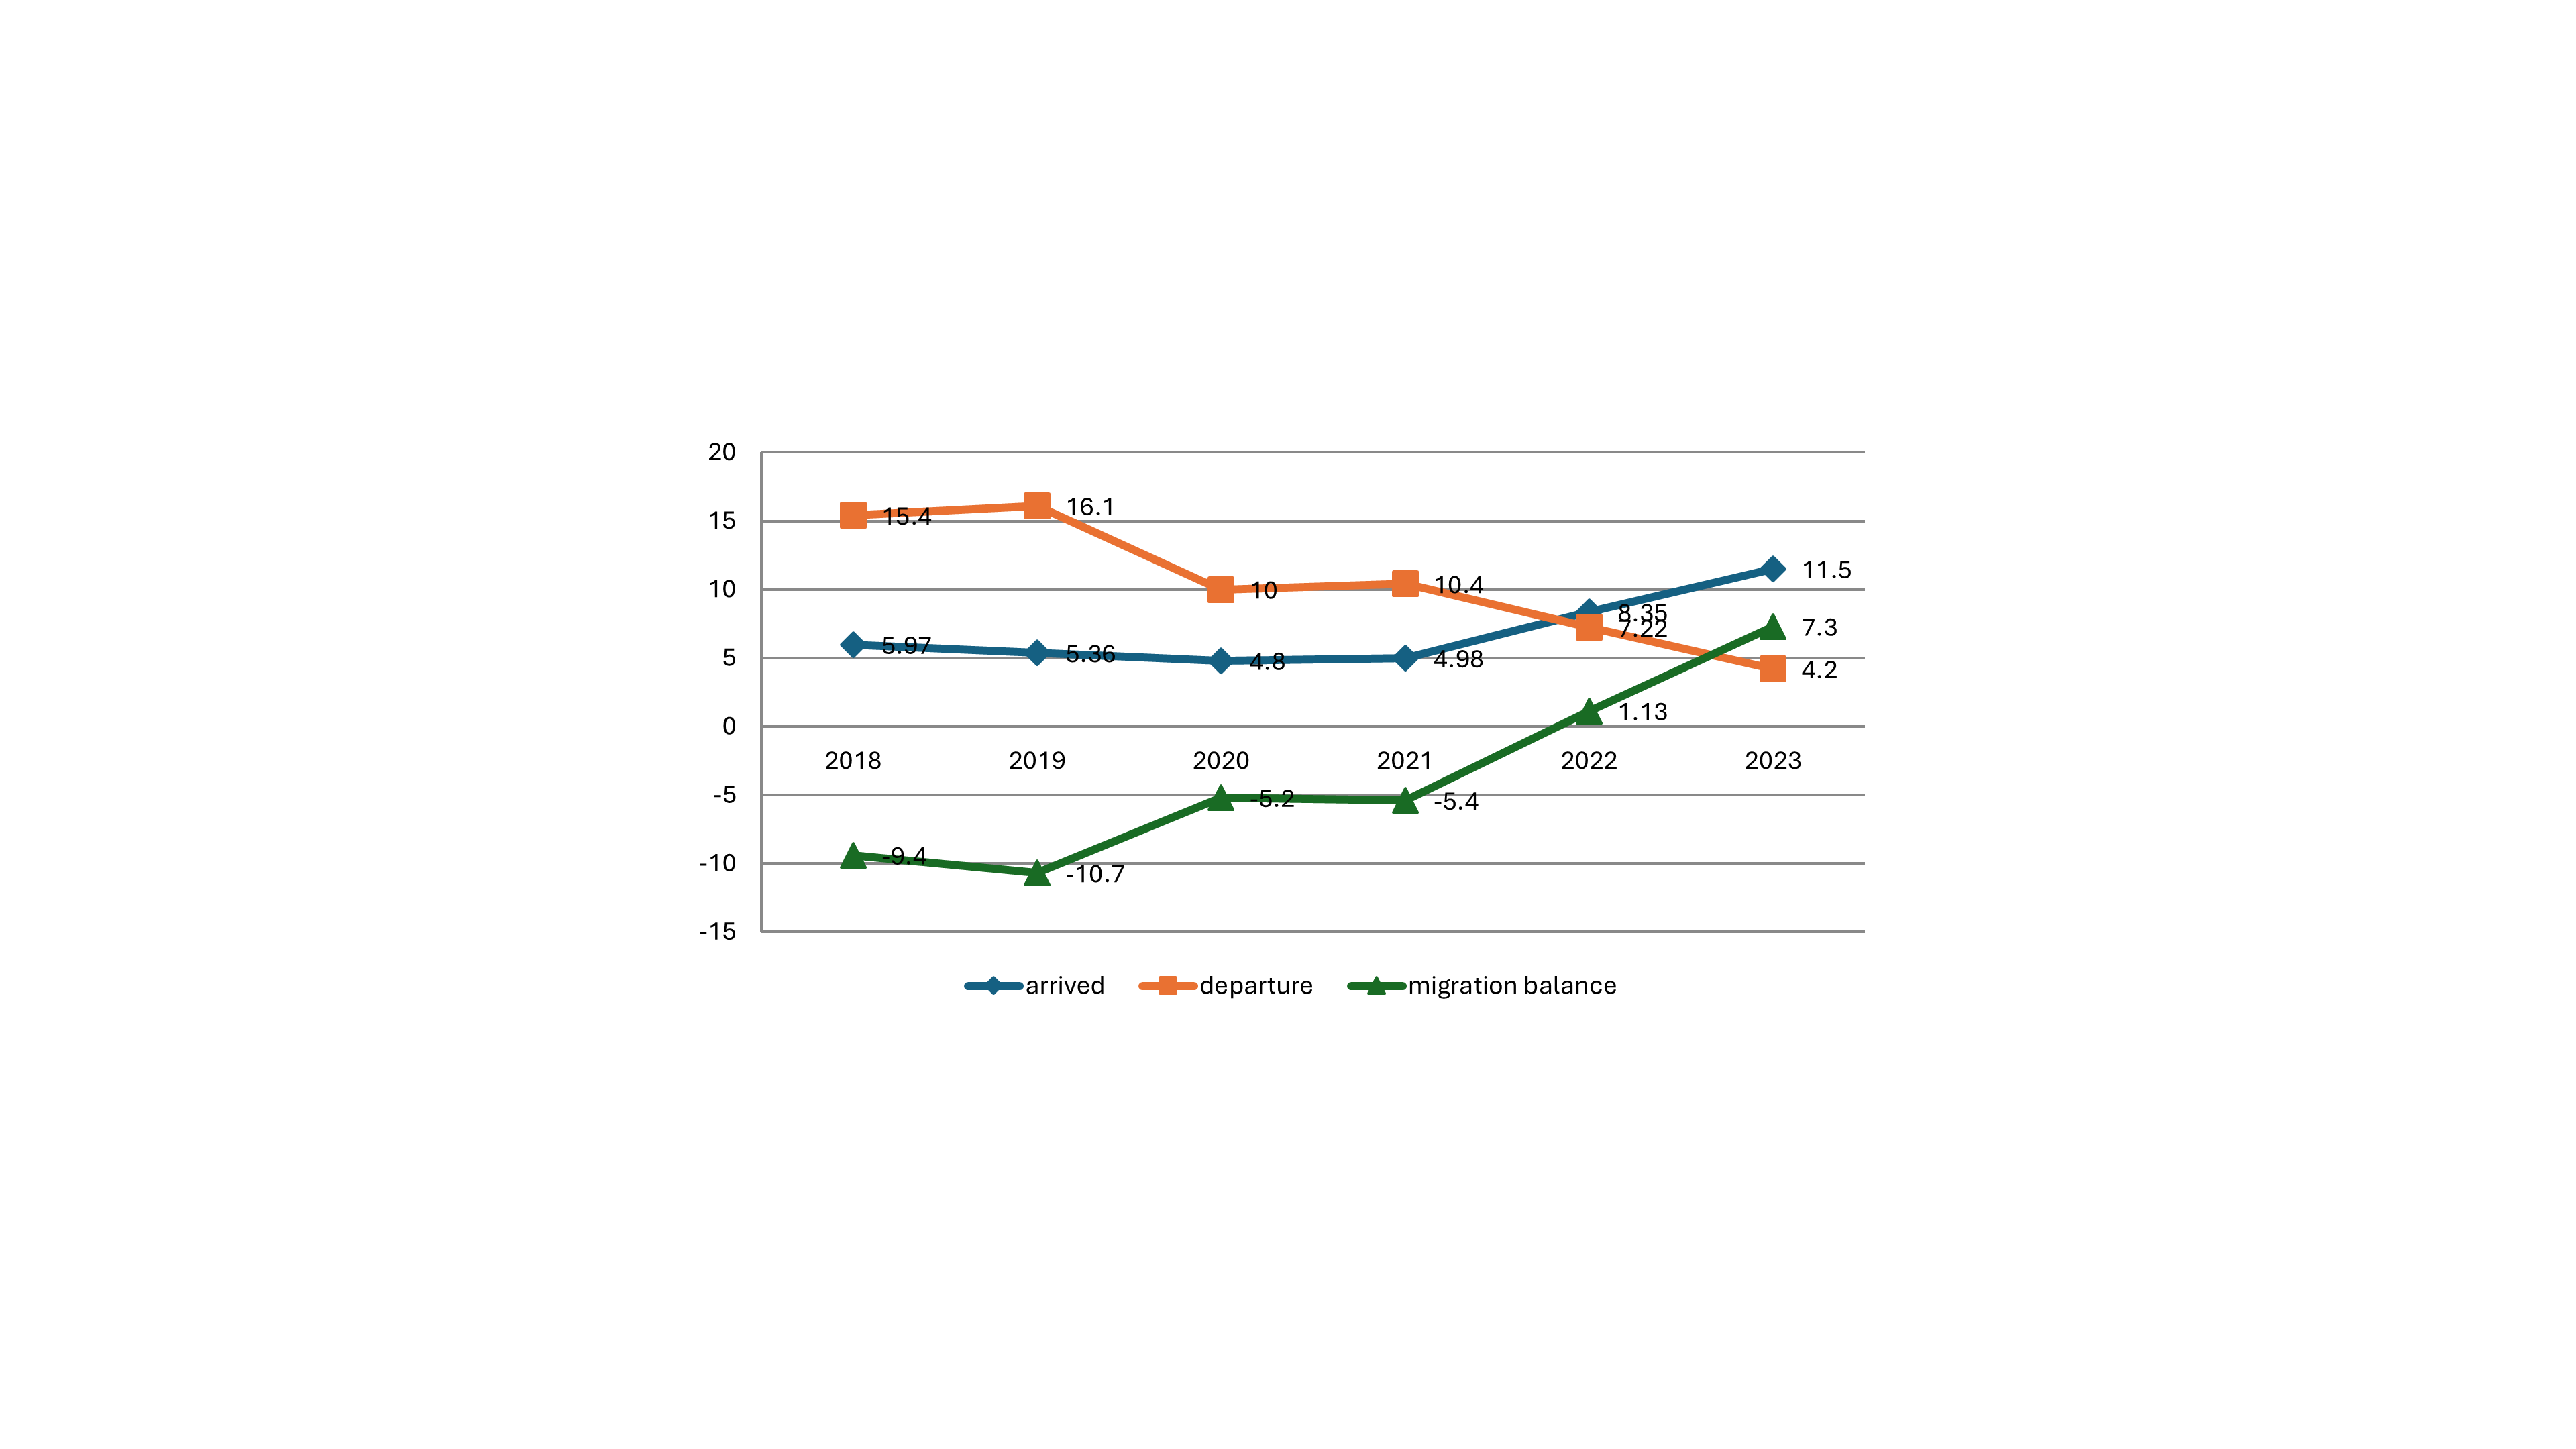
\includegraphics[width=0.7\textwidth]{media/ekon/Graph_4}
	\caption*{Figure 1 - External migration of youth in Kazakhstan, thousand people (2018-2023 years) {[}13{]}}
	\caption*{(Source: Bureau of National statistics of the Republic of Kazakhstan)}
\end{figure}

\begin{multicols}{2}
Analyzing the statistical data, from Figure 1 we see a decrease in the
emigration of young people from Kazakhstan in 2020 and 2022. First of
all, this is due to quarantine restrictions in the context of the
coronavirus pandemic and military actions in some countries. If in 2018
the number of people leaving was at the level of 15,355, then in 2020
this figure was 10017, in 2022- 7,222 people. At the same time, in 2023,
there is a flow of visitors to Kazakhstan, 38\% more young people
arrived during the year compared to the same period last year, or 11.5
thousand people to 8.35 thousand people. For the first time in many
years, the migration balance has flowed into a positive zone -- plus
4,000 young people. Most of the young people came from Russia {[}4,
13{]}.Youth migration is a separate independent area of research,
primarily because of its connection with education. The focus of
attention is gradually shifting to the youngest ages - to the period
when the initial decision to migrate in order to receive education is
made. Such a decision has a tremendous impact on both the subsequent
life of a young person and, in general, on the spatial distribution of
human capital. Often, youth educational migration becomes irreversible,
which weakens the labor markets of the regions from which young people
drop out.
\end{multicols}

\begin{figure}[H]
	\centering
	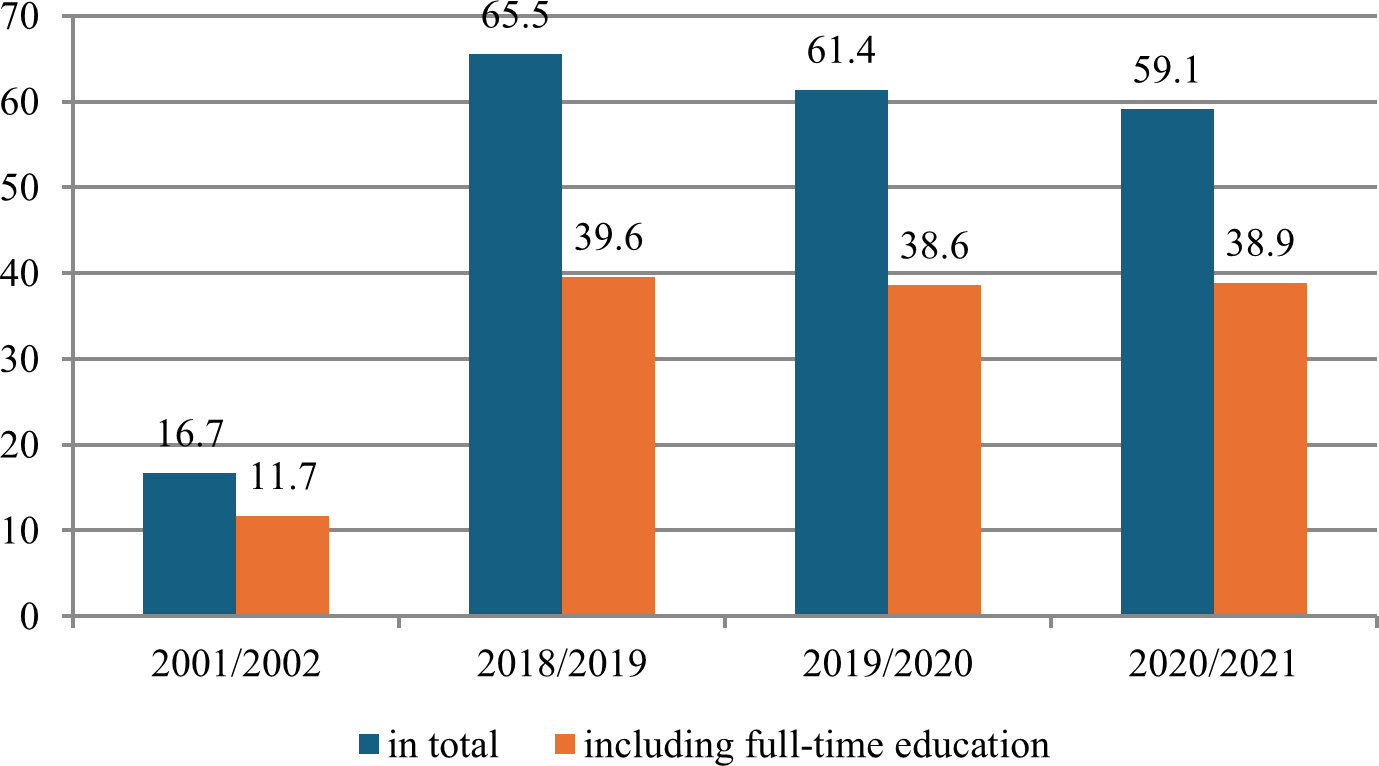
\includegraphics[width=0.7\textwidth]{media/ekon/Graph_5}
	\caption*{Figure 2 - The number of students from the Republic of Kazakhstan studying at universities of the Russian Federation, thousand people {[}14{]}}
\end{figure}

\begin{multicols}{2}
The main direction of educational migration from Kazakhstan is the
Russian Federation. As can be seen from Figure 2, there is a tendency
for the country to decrease the number of people traveling to the
Russian Federation for educational purposes due to the coronavirus
pandemic {[}14{]}. Kazakhstan is pursuing an active policy of supporting
educational migration both through academic mobility within the
framework of the Bologna process and through the international
scholarship "Bolashak". Students are distinguished by high spatial
mobility and the greatest resource of information interaction with other
countries. They have experience of staying in Western countries: as
tourists, earning money during summer vacations, and most thoroughly as
students. Many Kazakhstani students in the process of studying abroad
are actively looking for a future job.

As part of this research, 16 in-depth interviews were taken. Interviews
were conducted remotely with 11 women and 5 men. The youngest
interviewee is 21 years old, the oldest is 38 years old. 11 young people
had university degrees and 4 interviewers had postgraduate degrees. All
interviewees moved from 2010 to 2019. And at the time of the
conversation, they lived in countries such as the United States (12
people), the United Arab Emirates, the Netherlands, Australia, the
United Kingdom (one person each).

At the beginning of each interview, a general question was asked: "What
were the reasons for moving, why did you move?" The interviewees named
such reasons. One of the interviewees answered briefly and succinctly:
"Because there are much more prospects in the States than in
Kazakhstan." One of the interviewed girls briefly described the reasons
for moving to the USA: ``International environment, opportunity to
practice the language, more opportunities for development''. They also
highlighted the key attraction factors for moving, for example, to the
United States: ``Public services are working. Medicine heals. The police
are protecting. Taxes are spent on landscaping. The standard of living
is more uniform across the country. " Among girls, in most cases, the
decision to move was made by the husband. For example, quotes from girls
about the reasons for moving: ``My husband got a job in the Netherlands.
I plan to enroll in courses for another specialty. You need to retrain
to be someone in order to get a job. " Another girl' s
reason for moving was a marriage proposal: ``Because I received a
marriage proposal from a friend of mine in the United States. At the
same time, regardless of this, not knowing the intentions of my friend,
I was looking for an opportunity to leave the country, because in my 4th
year I studied in Japan for half a year, visited Korea and I wanted to
see the world further''. Man, 28 ``I wanted to do science, I was looking
for educational programs in the West. The decision to move was made
quickly after I learned the results of the interview for admission to
the magistracy''.

In conclusion, the interviewees were asked the questions "Is it possible
for your return to your homeland after emigration?". The majority wanted
the push factors that led to the move to change in Kazakhstan. For
example: "Yes, if she will respond to my wishes". "At this stage, no,
because in my opinion the country is economically ruined". "I may return
to Kazakhstan if the minimum wage, health care, the general quality of
life in the country and, probably, the government, which cares about the
people, change."

Thus, we can conclude that, according to 16 interview participants, the
key pushing factors in the political sphere are: corruption, tribalism.
In the social sphere: poorly developed social infrastructure (education,
healthcare), strong differentiation of the population by income level,
lack of opportunities for professional and career growth. In the legal
sphere: the lack of work of laws in practice. In the economic sphere:
economic crisis, unemployment, low wages, lack of normal working
conditions. It should be noted that the interviewees spoke about pushing
factors in an exaggerated form, i.e. talked about the problems existing
in Kazakhstan in an exaggerated form, confirming them with vivid
examples from life. The main pulling factors in the social sphere are: a
high standard of living, a functioning healthcare system, and the
absence of strong stratification in society in terms of income. The
interviewees chose countries such as the United States, the Netherlands,
the United Kingdom, and the UAE for further residence. A high standard
of living is a key attraction in these countries. Other factors were
also identified.

As for the costs of moving, in the social sphere, young specialists
faced such problems as the language barrier, the conflict of mentalities
and cultures, and ``culture shock''. In the legal field: obtaining a
visa and a residence permit. In the economic sphere: high prices for
goods and services, the difficulty of finding a job with a Kazakh
education. It is also worth noting how the interviewees told about the
difficulties of moving to another country. Despite the fact that there
were a lot of costs during the move and some coincide with push factors
from Kazakhstan, the majority tried to downplay the significance of
these negative memories by the moment of moving and move on to positive
events.

Along with the general Kazakhstani tendencies of youth migration, there
are regional features of their manifestation - in some regions the
migration attitudes towards leaving are high, in others they are less
significant.

The results of numerous studies in Kazakhstan and abroad show that the
process of transferring human capital across the borders of states is
inherently associated with international migration of the population,
which can be considered one of the few success factors that predetermine
the country' s ability to promote modernization, as well
as a source of transition to a new, more perfect , the stage of economic
development.

It is clear that migration processes can have both positive and negative
effects on the quality of human capital {[}15{]}. Obviously, the
migration inflow of the population expands the capabilities of the
recipient country not only in quantitatively replenishing the labor
force, but also in increasing knowledge, obtaining information
resources, contributing to the introduction of advanced technologies,
the application of advanced experience in organizing and managing
production and services. In modern conditions, when the choice of human
civilization in favor of the post-industrial perspective of the
development of society has become a reality, human capital, including
those brought in from the outside, becomes one of the most important
determinants of the formation and development of an innovative economy
of any state. Its accumulation predetermines an increase in the quality
of labor resources, as it increases the share of the ``component of
knowledge'' and the so-called ``complex labor force'' in them, which has
the ability to intellectual, creative work. In contrast, the function of
a simple labor force is performing labor activity {[}16{]}.

Speaking about the effects of large-scale labor migration, both on a
temporary and permanent basis, special attention should be paid to the
``brain drain'' for the human capital of the donating countries. It
should be noted that in many respects the consequences of the departure
of highly skilled labor depend on the level of development of the state
and the state of the national economy. For example, the departure of
scientists from the United States to other countries of the world does
not have a significant impact on the development of science in the
country. Scientific cadres are reproduced, talented scientists from all
over the world move to America every year. In this case, we should not
talk about the "brain drain", but about the circulation of scientists.
The opposite situation was observed in Kazakhstan in the early 90s, when
the mass departure of scientists and engineers blew out entire branches
of economic activity and scientific directions.

The return of young migrants to their home country can be an important
factor for the development of human capital and economic growth in the
country. Returning migrants often bring with them capital, ideas and
international connections, which contributes to the development of small
and medium-sized businesses. They can introduce innovations that have
been successfully implemented abroad. Studying abroad and working in
innovative sectors allows migrants to bring advanced technologies and
working methods. This is especially important for developing countries
seeking to close the technology gap. To strengthen the contribution of
young migrants, States can develop programs that help migrants return to
their homeland by providing support in finding employment, starting a
business and adapting.

{\bfseries Conclusion.} Migration theories must also take into account
educational migration, a period of increased investment in human
capital, when considering youth migration. The variability of life paths
in migration experience has received limited empirical justification,
and migration in the field of education should be considered as one of
the ways in which families continue to invest in the future productivity
of their children.

The key areas of Kazakhstan' s activity in the migration
sphere are fixed in the Concept of the Migration Policy of the Republic
of Kazakhstan for 2023-2027, which states that ``Kazakhstan adheres to
the strategy of temporary migration to involve foreign workers, optimal
settlement of the population throughout the country, as well as
long-term permanent migration in relation to ethnic repatriates arriving
in the Republic of Kazakhstan {[}17{]}. As a result, we can single out
one of the tasks of managing migration processes: the priority
attraction of highly qualified foreign specialists and the
implementation of a nationwide training program, which will ensure the
development of human capital.

Youth migration from Kazakhstan is driven by socio-economic, political,
and legal factors. The country faces significant push factors, such as
corruption, poor social services, and economic instability, leading to
an outflow of young, educated individuals seeking better opportunities
abroad. To reduce youth migration and develop human capital,
comprehensive reforms are needed. These should focus on improving living
and working conditions in the country, investing in education and
science, creating programs to retain and attract young people back, and
fostering regional development. Achieving these goals requires
collaboration between the government, businesses, and society, as well
as long-term investments in the potential of youth. The
government' s migration policy focuses on attracting
highly qualified specialists and enhancing national human capital
through strategic training programs, highlighting the importance of
managing migration processes effectively.
\end{multicols}

\begin{center}
{\bfseries References}
\end{center}

\begin{references}
1. McKenzie D. J. A profile of the world's young developing country
international migrants // Population and Development Review. -2008.-
Vol.34(1).- P.115 - 135. DOI 10.1111/j.1728-4457.2008.00208.x

2. Taylor, L. New Frontiers, Uncertain Futures: Migrant Youth and
Children of Migrants in a Globalised World // Background Paper for
Zurich. -2007.- 46 p.

3. Zakon RK «O gosudarstvennoj molodezhnoj politike» ot 9 fevralya 2015
goda №285-V. URL: \\\href{https://adilet.zan.kz/rus/docs/Z1500000285}{https://adilet.zan.kz} {[}In
Russian{]}.- Date of address: 11.10.2024

4. Molodezh'{} Kazakhstanа: statisticheskij sbornik,
2018-2022. {[}Youth of Kazakhstan : statistical \\compendium 2018-2022{]}.
Astana: Natsional' noe byuro statistiki Ministerstva
natsional' noj ekonomiki Respubliki Kazakhstan. URL:
https://stat.gov.kz/api/iblock/element/184021/file/ru/ - 2023. -164 s.
{[}In Russian{]}. - Date of address: 11.10.2024

5. Kurchidis K. V. Otsenka chistoj stoimosti chelovecheskogo kapitala
{[}Assessment of the Net Value of Human Capital{]} // Yaroslavskij
pedagogicheskij vestnik. -2011. -№ 2. -T.I {[}In Russian{]}.

6. Chiswick, B. The Effect of Americanization on the Earnings of
Foreign-born Men // Journal of Political Economy.-1978.-
Vol.86(5)-P.897-921.
\href{https://econpapers.repec.org/scripts/redir.pf?u=http\%3A\%2F\%2Fdx.doi.org\%2F10.1086\%2F260717;h=repec:ucp:jpolec:v:86:y:1978:i:5:p:897-921}{DOI
10.1086/260717}~

7. Kolosnicyna M.G., Suvorova I.K. Mezhdunarodnaja trudovaja migracija:
teoreticheskie osnovy i politika regulirovanija//Jekonomicheskij zhurnal
VShJe.-2005.-T.9 (4).-S.543-565.{[}In Russian{]}.

8. Massey, D. S. et al. Theories of International Migration: A Review
and Appraisal {[}Teorii mezhdunarodnoj migratsii: Obzor i otsenka{]} //
Population and Development Review. 1993. -Vol. 19(3). -P. 431-466. DOI
10.2307/2938462

9. Palalic, R., Durakovic, B., Ramadani, V., Ferreira, J.J.M. Human
capital and youth emigration in the ``new normal'' // Thunderbird
International Business Review. -2023. -Vol. 65(1). -P.49-63. DOI\\
10.1002/tie.22250

10. Lulle, A., Janta, H., Emilsson, H. Introduction to the Special
Issue: European youth migration: human capital outcomes, skills and
competences // Journal of Ethnic and Migration Studies. -2019. -Vol.47
(8). -P.1725-1739. DOI 10.1080/1369183X.2019.1679407.

11. Doumas, K., Avery, H. Lives `on hold' in Europe: an explorative
review of literature on youth aspirations and futures in situations of
migration and mobility // Eur J Futures Res. -2024. -Vol. 12(1). DOI\\
10.1186/s40309-023-00225-x

12. Molodezh'{} Kazakhstanа: statisticheskij sbornik,
2014-2018. {[}Youth of Kazakhstan : statistical \\compendium 2014-2018{]}.
Nur-Sultan: Komitet po statistike Ministerstva
natsional' noj ekonomiki \\Respubliki Kazakhstan, 2019. 185
s. URL: \href{https://stat.gov.kz/api/iblock/element/184021/file/ru/}{https://stat.gov.kz}-

Date of address: 15.11.2024. {[}In Russian{]}.

13. Molodezh'{} Kazakhstanа: statisticheskij sbornik,
2019-2023. {[}Youth of Kazakhstan : statistical \\compendium 2019-2023{]}.
Astana: Natsional' noe byuro statistiki Ministerstva
natsional' noj ekonomiki Respubliki Kazakhstan. - 2024.
-141 s. -Date of address: 15.11.2024{[}In Russian{]}.
\href{https://stat.gov.kz/api/iblock/element/184021/file/ru/}{https://stat.gov.kz}

14. Rossiya v cifrah. 2020: Kratkij statisticheskij sbornik. -M.:
Rosstat, 2020. -550 s. ISBN 978-5-89476-488-7 {[}In Russian{]}.

15. Volodin, V.M., Volodina, N.V., Pitaykina, I.A. Vliyanie processov
trudovoj migratsii na kachestvo chelovecheskogo kapitala RF // Vestnik
Dagestanskogo gosudarstvennogo tekhnicheskogo universiteta.
Tekhnicheskie nauki. -2017. -Vol. 44(1). -P. 173-185. DOI
10.21822/2073-6185-2017-44-1-173-185 {[}In Russian{]}.

16. Kirpichev, V. V. (n.d.) Transgranichnye migratsii naseleniya kak
istochnik vosproizvodstva trudovyh resursov i faktor nakopleniya
chelovecheskogo kapitala. URL:
\href{https://cyberleninka.ru/article/n/transgranichnye-migratsii-naseleniya-kak-istochnik-vosproizvodstva-trudovyh-resursov-i-faktor-nakopleniya-chelovecheskogo-kapitala}{https://cyberleninka.ru}.
{[}In Russian{]}.

17. Kontseptsiya migratsionnoj politiki na 2023-2027 gody. - 30.11.2022.
№ 961.URL: \href{https://adilet.zan.kz/rus/docs/P2200000961}{https://adilet.zan.kz} {[}In Russian{]}.
\end{references}

\begin{authorinfo}
\emph{{\bfseries Information about the author}}

Zhumashbekova S. K. - MSc, senior lecturer of Shakarim University,
Semey, Kazakhstan, e-mail:
\href{mailto:samalzhk@mail.ru}{\nolinkurl{samalzhk@mail.ru}};

Bayadilova B. M. - PhD, senior lecturer of K. Kulazhanov Kazakh
University of Technology and Business, Astana, Kazakhstan, e-mail:
\href{mailto:melisovna@mail.ru}{\nolinkurl{melisovna@mail.ru}};

Koichubayev A. S. - PhD, senior lecturer of Alikhan Bokeikhan
University, Semey, Kazakhstan, e-mail:\\
\href{mailto:koichubayev.a@abu.edu.kz}{\nolinkurl{koichubayev.a@abu.edu.kz}}

\emph{{\bfseries Сведения об авторах}}

Жумашбекова С. К. - магистр, старший преподаватель Университет им.
Шакарима, Семей, Казахстан, e-mail:\\
\href{mailto:samalzhk@mail.ru}{\nolinkurl{samalzhk@mail.ru}};

Баядилова Б. М.- PhD, старший преподаватель Казахский университет
технологии и бизнеса им. К.Кулажанова, Астана, Казахстан, e-mail:
\href{mailto:melisovna@mail.ru}{\nolinkurl{melisovna@mail.ru}};

Койчубаев А. С. - PhD, старший преподаватель Alikhan Bokeikhan
University, Семей, Казахстан, e-mail:\\
\href{mailto:koichubayev.a@abu.edu.kz}{\nolinkurl{koichubayev.a@abu.edu.kz}}
\end{authorinfo}
